	\documentclass[11pt]{book}
	
	\usepackage{amsfonts,amsthm, bm,amsmath, bbm,amssymb,mathtools}
	\usepackage{fullpage}
	\usepackage{tikz, pgfplots} % added for Lecture 2	
	\usepackage{float}  % added for Lecture 8
	
	\newtheorem{theorem}{Theorem}[chapter]
	\newtheorem{lemma}[theorem]{Lemma}
	
	\theoremstyle{definition}
	\newtheorem{definition}[theorem]{Definition}
	\newtheorem{example}[theorem]{Example}
	\newtheorem{xca}[theorem]{Exercise}
	\newtheorem{corollary}[theorem]{Corollary}  % added for Lecture 5
	\newtheorem{proposition}{Proposition}[section]  % added for Lecture 6
		
	\theoremstyle{remark}
	\newtheorem{remark}[theorem]{Remark}
	
	\numberwithin{section}{chapter}
	\numberwithin{equation}{chapter}
	
	\makeindex
	
	\def\lectureformat{1}
	\usepackage{color}
\usepackage{lipsum}

\ifnum\lectureformat=1
\newcommand{\metadata}[3]
{
	\newpage
	
	\def\lectureID{#1}
	
	\setcounter{chapter}{\lectureID}

%	\draftnotice
	
	\begin{center}
		\bf\large CS229M/STATS214: Machine Learning Theory
	\end{center}
	
	\noindent
	Lecturer: Tengyu Ma   %%% FILL IN LECTURER (if not RS)
	\hfill
	Lecture \# \lectureID              %%% FILL IN LECTURE NUMBER HERE
	\\
	Scribe: #2                  %%% FILL IN YOUR NAME HERE
	\hfill
	#3           %%% FILL IN LECTURE DATE HERE
	
	\noindent
	\rule{\textwidth}{1pt}
	
	\medskip
}
\else 
\newcommand{\metadata}[3]{}
\fi

\newcommand*\circled[1]{\tikz[baseline=(char.base)]{
	\node[shape=circle,draw,inner sep=2pt] (char) {#1};}}

\DeclareMathOperator*{\Exp}{\mathbb{E}}
\DeclareMathOperator*{\argmin}{\textup{argmin}}
\DeclareMathOperator*{\argmax}{\textup{argmax}}

\newcommand{\Cov}{\operatorname{Cov}}
\newcommand{\KL}{\operatorname{KL}}
\newcommand{\margin}{\text{margin}}
\newcommand{\poly}{\operatorname{poly}}
\newcommand{\sd}{\operatorname{sd}}
\newcommand{\sgn}{\text{sgn}}
\newcommand{\tr}{\operatorname{tr}}
\newcommand{\Var}{\operatorname{Var}}

\newcommand{\err}{\ell_{\textup{0-1}}}
\newcommand{\Err}{L_{\textup{0-1}}}
\newcommand{\thetaerm}{\theta_{\textup{ERM}}}
\newcommand{\hatL}{\widehat{L}}
\newcommand{\tilO}{\widetilde{O}}
\newcommand{\iid}{\overset{\textup{iid}}{\sim}}
\newcommand\defeq{\stackrel{\mathclap{\tiny \mbox{$\Delta$}}}{=}}

\newcommand{\norm}[1]{\|#1\|}
\newcommand{\Norm}[1]{\left\|#1\right\|}
\renewcommand{\l}{\left}
\renewcommand{\r}{\right}
\newcommand{\rbr}[1]{\left(#1\right)}
\newcommand{\sbr}[1]{\left[#1\right]}
\newcommand{\cbr}[1]{\left\{#1\right\}}
\newcommand{\abs}[1]{\left\lvert#1\right\rvert}
\newcommand{\inprod}[1]{\left\langle#1\right\rangle}

\newcommand{\al}[1]{
	\begin{align}
	#1
	\end{align}
}

\renewcommand{\sp}[1]{^{(#1)}}

\newcommand{\cA}{\mathcal A}
\newcommand{\cB}{\mathcal B}
\newcommand{\cC}{\mathcal C}
\newcommand{\cD}{\mathcal D}
\newcommand{\cE}{\mathcal E}
\newcommand{\cF}{\mathcal F}
\newcommand{\cG}{\mathcal G}
\newcommand{\cH}{\mathcal H}
\newcommand{\cI}{\mathcal I}
\newcommand{\cJ}{\mathcal J}
\newcommand{\cK}{\mathcal K}
\newcommand{\cL}{\mathcal L}
\newcommand{\cM}{\mathcal M}
\newcommand{\cN}{\mathcal N}
\newcommand{\cO}{\mathcal O}
\newcommand{\cP}{\mathcal P}
\newcommand{\cQ}{\mathcal Q}
\newcommand{\cR}{\mathcal R}
\newcommand{\cS}{\mathcal S}
\newcommand{\cT}{\mathcal T}
\newcommand{\cU}{\mathcal U}
\newcommand{\cV}{\mathcal V}
\newcommand{\cW}{\mathcal W}
\newcommand{\cX}{\mathcal X}
\newcommand{\cY}{\mathcal Y}
\newcommand{\cZ}{\mathcal Z}

\newcommand{\bbB}{\mathbb B}
\newcommand{\bbS}{\mathbb S}
\newcommand{\bbR}{\mathbb R}
\newcommand{\bbZ}{\mathbb Z}
\newcommand{\bbI}{\mathbb I}
\newcommand{\bbQ}{\mathbb Q}
\newcommand{\bbP}{\mathbb P}
\newcommand{\bbE}{\mathbb E}
\newcommand{\bbN}{\mathbb N}

\newcommand{\E}{\mathbb{E}}
\newcommand{\N}{\mathbb{N}}
\newcommand{\R}{\bbR}
\newcommand{\Z}{\mathbb{Z}}


% for course staff to edit or comment
\def\shownotes{1}  %set 1 to show author notes
\ifnum\shownotes=1
\newcommand{\authnote}[2]{[#1: #2]}
\else
\newcommand{\authnote}[2]{}
\fi
\newcommand{\tnote}[1]{{\color{blue}\authnote{TM}{#1}}}

% for long term comments 
\def\shownotes{0}  %set 1 to show author notes
\ifnum\shownotes=1
\newcommand{\authnotelong}[2]{[#1: #2]}
\else
\newcommand{\authnotelong}[2]{}
\fi
\newcommand{\tnotelong}[1]{{\color{blue}\authnotelong{TM}{#1}}}
	\begin{document}
	
	\frontmatter
	
	\mainmatter
	\let\sec\section
	\let\subsec\subsection
	
	\newcommand{\secwarning}[1]{
		{	
			\color{red}
			$\backslash$section and $\backslash$subsection are disallowed, please use 	$\backslash$sec and $\backslash$subsec instead
		}
	}
	\let\section\secwarning
	\let\subsection\secwarning
	
	
	\newcommand{\draftnotice}{\vbox to 0.25in{\noindent
			\raisebox{0.6in}[0in][0in]{\makebox[\textwidth][r]{\it
					DRAFT --- a final version will be posted shortly}}}
		\vspace{-.25in}\vspace{-\baselineskip}
	}
	
	%\section{}
	
% reset section counter
\setcounter{section}{0}

%\metadata{lecture ID}{Your names}{date}
\metadata{11}{Andrew Wang}{Feb 22nd, 2021}

\sec{Review and overview}

Last lecture, we discussed the role of optimization in understanding deep learning model generalization. In particular, gradient descent cannot always find the global minimum for a non-convex loss function. However, there are some special problems where (i) gradient descent can find a local minimum, and (ii) all local minima are also global minima. For these problems, gradient descent is able to find a global minimum. Based on these observations, we began carrying out a two step plan:
\begin{enumerate}
\item Characterize the set of functions for which gradient descent can find a global minimum, then
\item Identify machine learning problems that belong to this set.
\end{enumerate}

We proved that principal component analysis (PCA) belongs in this set of problems (all local minima are global minima), and began proving a similar approximate claim for matrix completion. In this lecture, we finish this proof and begin discussing a new topic, the Neural Tangent Kernel (NTK), which will give further insights into local minima near a given initialization.

\sec{Matrix completion \cite{ge2016}}
Recall problem of rank-1 matrix completion problem. Let $M = zz^T$ be a rank-1 symmetric, positive semi-definite matrix for some $z \in \mathbb{R}^d$ such that $\norm{z}_2 = 1$ and $\norm{z}_\infty \leq \mu / \sqrt{d}$. We observe random entries of $M$ and must recover the remaining entries.

\begin{definition}
Suppose $M\in \bbR^{d\times d}$ and $\Omega \subseteq [d] \times [d]$. We define $P_{\Omega}(M)$ to be the matrix obtained by zeroing out every entry outside $\Omega$. 
\end{definition}

\begin{definition}[Matrix completion]
Suppose $M\in \bbR^{d\times d}$ and every entry of $M$ is included in $\Omega$ with probability $p$. The \textit{matrix completion task} is to recover $M$ (with respect to some loss function) given the observation $P_{\Omega}(M)$.
\end{definition}

In order to solve the matrix completion problem, one can search for $x$ that locally minimizes the following objective:

\begin{equation}
f(x) = \frac{1}{2}\norm{P_\Omega(M-xx^T)}_F^2 = \frac{1}{2} \sum_{(i,j) \in \Omega} (M_{ij} - x_ix_j)^2.
\end{equation}

The goal is to prove that local minima of this objective function are close to a global minimum:

\begin{theorem}\label{lec11:thm:matrix-completion}
Assume $p = \dfrac{\textrm{poly}(\mu, \log d)}{d\epsilon^2}$. Then with high probability, all local minima of $f$ are $O(\sqrt{\epsilon})$-close to $+z$ or $-z$ (the global minima of $f$).
\end{theorem}

Before presenting the proof, we make some observations that will guide the proof strategy.

\begin{remark}
$f(x)$ can be viewed as a sampled version of the PCA loss function $g(x) = \frac{1}{2}\norm{M - xx^T}_F^2 = \frac{1}{2}\sum_{(i,j) \in [d]\times[d]} (M_{ij} - x_ix_j)^2$, in which we only observe a subset of the matrix entries. Thus, we would like to claim that $f(x) \approx g(x)$. However, matching the values of $f$ and $g$ is not sufficient to prove the theorem: even a small margin of error between $f$ and $g$ could lead to creation of many spurious local minima (see Figure~\ref{lec11:fig:matrix_completion_f_g} for an illustration). In order to ensure that the local minima of $f$ look like the local minima of $g$, we will need further conditions like $\nabla f(x) \approx \nabla g(x)$ and $\nabla^2 f(x) \approx \nabla^2 g(x)$.
\end{remark}

\begin{figure}
    \centering
    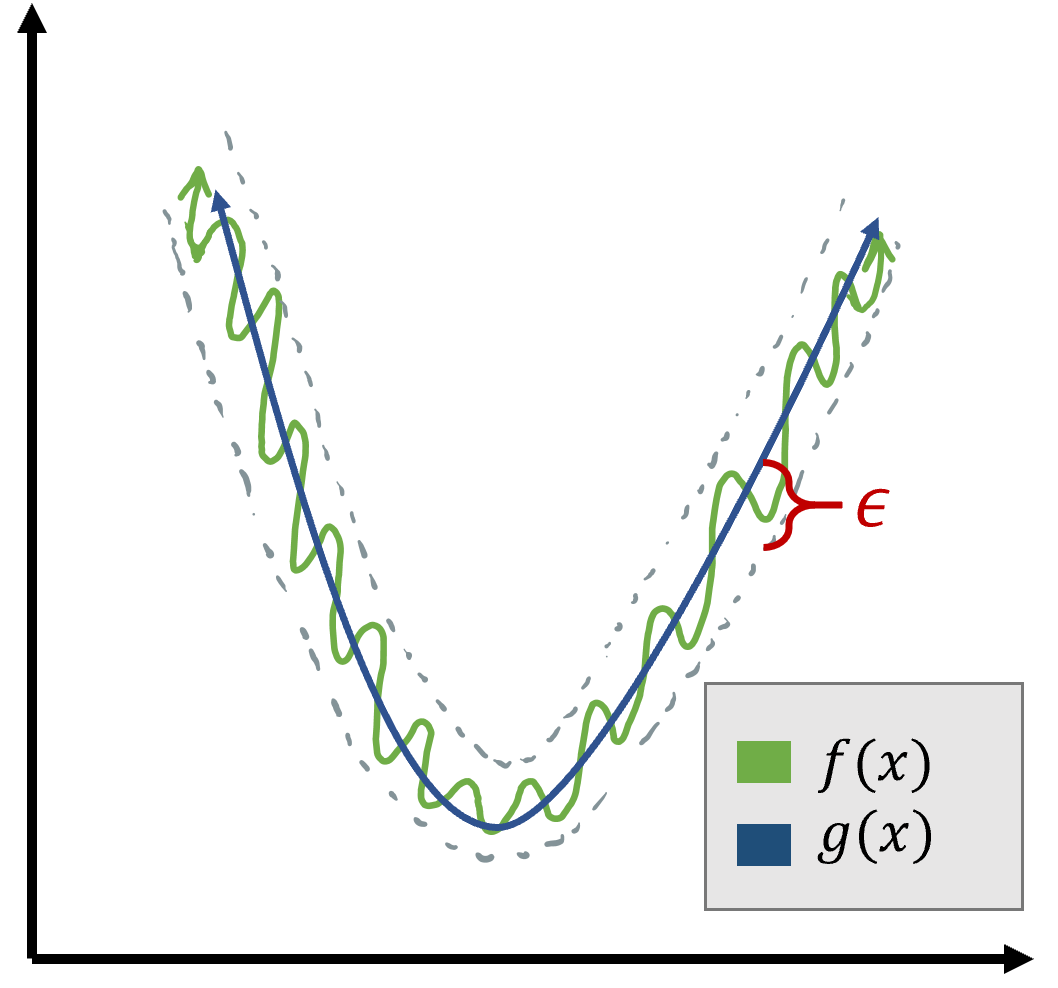
\includegraphics[width=2.5in]{figures/matrix-completion-f-g.png}
    \caption{Even if $f(x)$ and $g(x)$ are no more than $\epsilon$ apart at any given $x$, the local minima of $f$ may look dramatically different from the local minima of $g$.}
    \label{lec11:fig:matrix_completion_f_g}
\end{figure}

\begin{remark}
Key idea: concentration for scalars is easy. We can approximate a sum of scalars via a sample:
\begin{equation}
\sum_{(i,j) \in \Omega} T_{ij} \approx p\sum_{(i,j) \in [d]\times[d]} T_{ij},
\end{equation}
where we use $\approx$ to mean that
\begin{equation}
\Bigl| \sum_{(i,j) \in \Omega} T_{ij} - p\sum_{(i,j) \in [d]\times[d]} T_{ij} \Bigr| < \epsilon
\end{equation}
with high probability. This suggests the strategy of casting the estimation of our desired quantities in the form of estimating a scalar sum via a sample. In particular, we note that for any matrices $A$ and $B$,
\begin{equation}
\langle A, P_\Omega(B) \rangle = \sum_{(i,j) \in \Omega} A_{ij}B_{ij} \approx p\langle A, B \rangle.
\end{equation}
\end{remark}

To make use of this observation to understand the quantities of interest ($\nabla f(x)$ and $\nabla^2 f(x)$), we compute the bilinear and quadratic forms for $\nabla f(x)$ and $\nabla^2 f(x)$ respectively:
\begin{equation}
\langle v, \nabla f(x) \rangle = \langle v, P_\Omega(M-xx^T)x \rangle = \langle vx^T, P_\Omega(M-xx^T) \rangle,
\end{equation}
where we have used the fact that $\langle A,BC \rangle = \langle AC^T,B\rangle$. Also note that $vx^T$ is a rank-1 matrix and $M-xx^T$ is a rank-2 matrix.
\begin{align}
\langle v, \nabla^2 f(x) v \rangle &= \norm{P_\Omega(vx^T + xv^T)}_F^2 - 2\langle P_\Omega(M-xx^T), vv^T \rangle \\
&=  \langle P_\Omega(vx^T + xv^T), vx^T + xv^T \rangle - 2\langle P_\Omega(M-xx^T), vv^T \rangle,
\end{align}

where we have used the fact that $\norm{P_\Omega(A)}_F^2 = \langle P_\Omega(A), P_\Omega(A)\rangle = \langle P(\Omega(A), A\rangle$.

The key lemma that applies the scalar concentration to these matrix quantities is as follows:

\begin{lemma}
Let $\epsilon>0$, $p = \dfrac{\textrm{poly}(\mu, \log d)}{d\epsilon^2}$. Given that $A = uu^T, B=vv^T$ for some $u, v$ satisfying $\norm{u}_2 \leq 1$, $\norm{v}_2 \leq 1$, $\norm{u}_\infty \leq \mu / \sqrt{d}$, $\norm{v}_\infty \leq \mu / \sqrt{d}$, we have $|\langle P_\Omega(A), B \rangle/p - \langle A, B\rangle| \leq \epsilon$ w.h.p.
\label{lec11:lem:concentration_lemma}
\end{lemma}

If we can show that $g$ has no bad local minima via a proof that only uses $g$ via terms of the form $\langle v, \nabla g(x) \rangle$ and $\langle v, \nabla^2 g(x) v \rangle$, then by Lemma~\ref{lec11:lem:concentration_lemma} this proof will automatically generalize to $f$ by concentration.

Next, we prove some facts about $g$ and show the analogous proofs for $f$ that we will use in the proof of Theorem~\ref{lec11:thm:matrix-completion}.

\begin{lemma}[Connecting inner product and norm for $g$]\label{lec11:lem:inner-g}
If $x$ satisfies $\nabla g(x) = 0$, then $\langle x,z \rangle^2 = \norm{x}_2^4$.
\end{lemma}

\begin{proof}
\begin{align}
    \nabla g(x) = 0 &\implies \langle x, \nabla g(x) \rangle = 0 \\
   & \implies \langle x, (zz^T-xx^T)x \rangle = 0 & (\because \nabla g(x) = (M - xx^T)x) \\
   & \implies \langle x,z \rangle^2 = \norm{x}_2^4.
\end{align}
\end{proof}

\begin{lemma}[Connecting inner product and norm for $f$]\label{lec11:lem:inner-f}
Suppose $\norm{x}_\infty \leq 2\mu / \sqrt{d}$. If $x$ satisfies $\nabla f(x) = 0$, then $\langle x,z \rangle^2 \geq \norm{x}_2^4 - \epsilon$ with high probability.
\label{inner_prod_norm_f}
\end{lemma}

\begin{proof}
\begin{align}
    \nabla f(x) = 0 &\implies \langle x, \nabla f(x) \rangle = 0 \\
    & \implies \langle x, \nabla g(x) \rangle \approx \langle x, \nabla f(x) \rangle/p \pm \epsilon & \text{(by Lemma \ref{lec11:lem:concentration_lemma})} \\
   & \implies |\langle x, (zz^T-xx^T)x \rangle| \leq \epsilon & \text{w.h.p.} \\
   & \implies \langle x,z \rangle^2 \geq \norm{x}_2^4 - \epsilon & \text{w.h.p.}
\end{align}
\end{proof}

\begin{lemma}[Bound norm for $g$]\label{lec11:lem:bound-g}
    If $\nabla^2 g(x) \succeq 0$, then $\norm{x}_2^2 \geq 1/3$.
\end{lemma}

\begin{proof}
\begin{align}
    \nabla^2 g(x) \succeq 0
    &\implies \langle z, \nabla^2 g(x)z\rangle \geq 0 \\
    &\implies \norm{zx^T + xz^T}_F^2 - 2z^T(zz^T-xx^T)z \geq 0 \\
    &\implies 1 \leq \norm{x}_2^2 + 2\langle x,z \rangle^2 \leq \norm{x}_2^2 + 2\norm{x}_2^2 = 3\norm{x}_2^2 &\text{(by Cauchy-Schwarz)} \\
    &\implies \norm{x}_2^2 \geq 1/3.
\end{align}
\end{proof}

\begin{lemma}[Bound norm for $f$]\label{lec11:lem:bound-f}
    Suppose $\norm{x}_\infty \leq \mu / \sqrt{d}$. If $\nabla^2 f(x) \succeq 0$, then $\norm{x}_2^2 \geq 1/3 - \epsilon/3$ with high probability.
\end{lemma}
\begin{proof}
\begin{align}
    \nabla^2 f(x) \succeq 0
    &\implies \langle z, \nabla^2 f(x)z \rangle \geq 0 \\
    &\implies \langle z, \nabla^2g(x)z \rangle \geq -\epsilon & \text{w.h.p. (by Lemma \ref{lec11:lem:concentration_lemma})} \\
    &\implies 3\norm{x}_2^2 \geq 1-\epsilon & \text{w.h.p.} \\
    &\implies \norm{x}_2^2 \geq 1/3 - \epsilon/3 & \text{w.h.p.}
\end{align}
\end{proof}

\begin{lemma}[$g$ has no bad local minimum]
    All local minima of $g$ are global minima.
\end{lemma}

\begin{proof}
\begin{align}
    \nabla g(x) = 0
    & \implies \langle z, \nabla g(x) \rangle = 0 \\
    & \implies \langle z, (zz^T-xx^T)x \rangle = 0 \\
    & \implies \langle x,z\rangle (1-\norm{x}_2^2) = 0.
\end{align}
Since $|\langle x,z \rangle| \geq 1/3 \neq 0$ (by Lemma~\ref{lec11:lem:bound-g}), we must have $\norm{x}_2^2 = 1$. But then Lemma~\ref{lec11:lem:inner-g} implies $\langle x, z\rangle^2 = \norm{x}_2^4 = 1$, so $x = \pm z$ by Cauchy-Schwarz.
\end{proof}

We now prove Theorem~\ref{lec11:thm:matrix-completion}, restated for convenience:
\begin{theorem}[$f$ has no bad local minimum]
Assume $p = \dfrac{\textrm{poly}(\mu, \log d)}{d\epsilon^2}$. Then with high probability, all local minima of $f$ are $O(\sqrt{\epsilon})$-close to $+z$ or $-z$.
\end{theorem}

\begin{proof}
Observe that $\norm{x-z}_2^2 = \norm{x}_2^2 + \norm{z}_2^2 - 2\langle x,z \rangle \leq \norm{x}_2^2 + 1 - 2\langle x,z \rangle$. Our goal is to show that this quantity is small with high probability, hence we need to bound $\norm{x}_2^2$ and $\langle x,z \rangle$ w.h.p. Note that the following bounds in this proof are understood to hold w.h.p.
    
Let $x$ be such that $\nabla f(x) = 0$. For $\epsilon \leq 1/16$,
\begin{align}
\langle x,z \rangle^2 &\geq \norm{x}_2^4 - \epsilon &\text{(by Lemma~\ref{lec11:lem:inner-f})} \\
&\geq (1/3-\epsilon/3)^2 - \epsilon &\text{(by Lemma~\ref{lec11:lem:bound-f})} \\
&\geq 1/32. \label{lec11:eqn:xz-bound}
\end{align}

With this, we can get a bound on $\norm{x}_2^2$:
\begin{align}
\nabla f(x) = 0 &\implies \langle x, \nabla f(x) \rangle = 0 \\
&\implies |\langle z, \nabla g(x) \rangle| \leq \epsilon & \text{(by Lemma \ref{lec11:lem:concentration_lemma})} \\
&\implies |\langle x,z\rangle| \cdot |1-\norm{x}_2^2| \leq \epsilon &\text{(by dfn of $g$)} \\
&\implies |1-\norm{x}_2^2| \leq 32\epsilon = O(\epsilon) &\text{(by \eqref{lec11:eqn:xz-bound})} \\
&\implies \norm{x}_2^2 = 1 \pm O(\epsilon). \label{lec11:eqn:xnorm-bound}
\end{align}
    
Next, we bound $\langle x,z \rangle$:
\begin{align}
\langle x, z \rangle^2 &\geq \norm{x}_2^4 - \epsilon &\text{(by Lemma \ref{inner_prod_norm_f})} \\
&\geq (1-O(\epsilon))^2 - \epsilon &\text{(by \eqref{lec11:eqn:xnorm-bound})} \\
&= 1 - O(\epsilon).
\end{align}

Finally, we put these quantities together to bound $\norm{x-z}_2^2$. We have two cases:
    
\textbf{Case 1}: $\langle x,z\rangle \geq 1 - O(\epsilon)$. Then
\begin{align}
\norm{x-z}_2^2 &= \norm{x}_2^2 + \norm{z}_2^2 - 2\langle x,z \rangle \\
&\leq \norm{x}_2^2 + 1 - 2\langle x,z \rangle \\
&\leq 1 + O(\epsilon) + 1 - 2(1-O(\epsilon)) \\
&\leq O(\epsilon).
\end{align} 
    
Hence we conclude $x$ is $O(\sqrt{\epsilon})$-close to $z$.
    
\textbf{Case 2}: $\langle x,z\rangle \leq -(1 - O(\epsilon))$. Then by an analogous argument, $x$ is $O(\sqrt{\epsilon})$-close to $-z$.
\end{proof}

We have shown above that matrix completion of a rank-1 matrix has no spurious local minima. This proof strategy can be extended to handle higher-rank matrices and noisy matrices \cite{ge2016}. The proof also demonstrates a generally useful proof strategy: often, reducing a hard problem to an easy problem results in solutions that do not give much insight into the original problem, because the proof techniques do not generalize. It can often be fruitful to seek a proof in the simplified problem that makes use of a restricted set of tools that could generalize to the harder problem. Here we limited ourselves to only using $\langle v, \nabla g(x)\rangle$ and $\langle v, \nabla^2 g(x) v\rangle$ in the easy case; these quantities could then be easily converted to analogous quantities in $f$ via the concentration lemma (Lemma~\ref{lec11:lem:concentration_lemma}).

\sec{Other problems where all local minima are global minima}
We have now demonstrated that two classes of machine learning problems, rank-1 PCA and rank-1 matrix completion, have no spurious local minima and are thus amenable to being solvable by gradient descent methods. We now outline some major classes of problems for which it is known that there are no spurious local minima.

\begin{itemize}
    \item Principal component analysis (covered in previous lecture).
    \item Matrix completion (and other matrix factorization problems). On a related note, it has also been shown that linearized neural networks of the form $y = W_1W_2x$, where $W_1$ and $W_2$ are optimized separately, have no spurious local minima \cite{baldi1989neural}. It should be noted that linearized neural networks are not very useful in practice since the advantage of optimizing $W_1$ and $W_2$ separately versus optimizing a single $W=W_1W_2$ is not clear.
    \item Tensor decomposition. The problem is as follows:
    \begin{align}
        \text{maximize }\quad \sum_{i=1}^d \sum_{j=1}^d \sum_{k=1}^d \sum_{l=1}^d T_{ijkl} x_ix_jx_kx_l \quad \text{such that } \quad \norm{x}_2 = 1.
    \end{align}
    Additionally, constraints are imposed on the tensor $T$ to make the problem tractable. For example, one condition is that $T$ must be a low-rank tensor with orthonormal components \cite{ge2015}.
\end{itemize}

In general, the loss landscapes of neural networks (with nonlinearities) is currently not as well understood, though we now introduce the \textit{neural tangent kernel} which allows us to make some characterizations of the loss near a given neural network initialization.

\sec{Neural tangent kernel (NTK) approach}
We now move to a new topic of the \textit{neural tangent kernel (NTK)}, which will give further insight into the loss landscape in the neighborhood of a given parameter initialization.

\begin{figure}
    \centering
    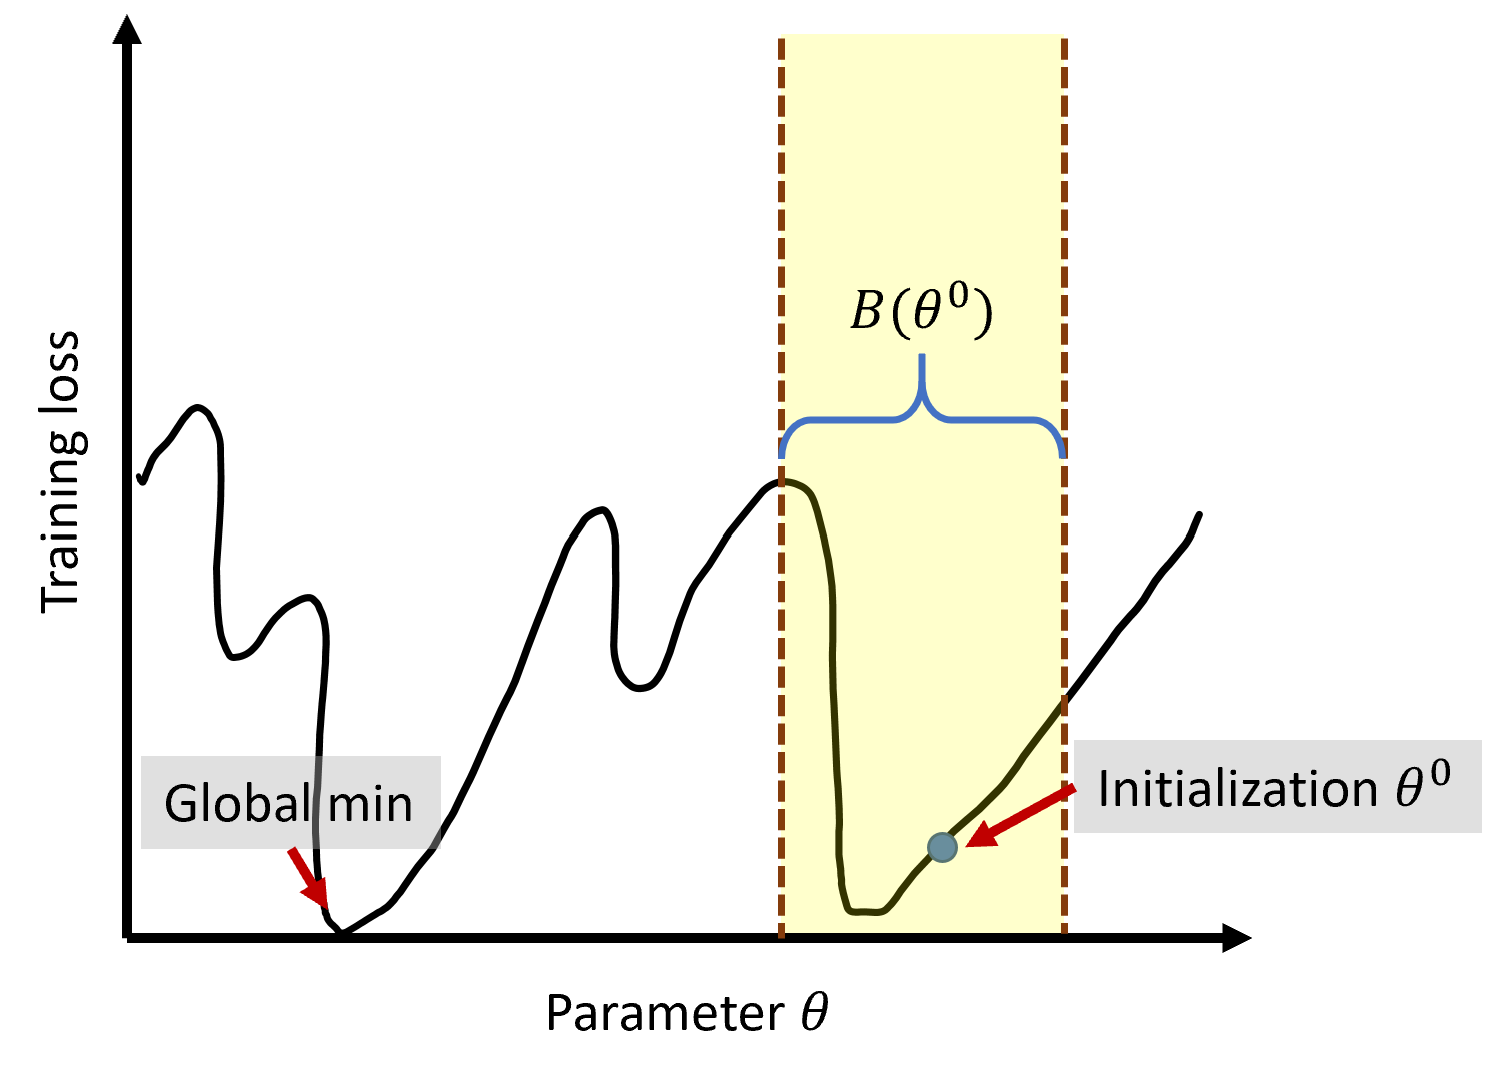
\includegraphics[width=2.5in]{figures/ntk-loss-landscape.png}
    \caption{The training loss landscape around a given parameter initialization $\theta^0$. We hope that the neighborhood around $\theta^0$ contains a local minimum that is close to the global minimum.}
    \label{lec11:fig:ntk_loss_landscape}
\end{figure}

The key insight of the NTK approach is that if we take an appropriate random parameter initialization $\theta^0$ (which we will choose later), we can identify a special neighborhood of $\theta^0$, denoted $B(\theta^0)$, where ``everything is nice''. That is, the function is convex in $B(\theta^0)$, there is a global minimum in the $B(\theta^0)$, and the algorithm starting at $\theta^0$ will converge to that global minimum. (See Figure~\ref{lec11:fig:ntk_loss_landscape} for an illustration.)


Take a random initialization $\theta = \theta^0$ and Taylor expand the loss around $\theta^0$ w.r.t. $\theta$:
\begin{align}
f_\theta(x) &= \underbrace{f_{\theta^0}(x) + \langle \nabla_\theta f_{\theta^0}(x), \theta - \theta^0 \rangle}_{g_\theta(x)} + O((\theta-\theta^0)^2).
\end{align}

In other words, we take the tangent plane to $f_\theta$ at $x$ (a linear approximation). We observe that $g_\theta$ is an affine function of $\theta$. Additionally, defining $\Delta \theta = \theta - \theta^0$, we see that the first term does not depend on $\Delta \theta$ while the second term $\langle \nabla_\theta f_{\theta^0}(x), \theta - \theta^0 \rangle$ is linear in $\Delta \theta$. (For convenience, we will sometimes choose to design $\theta^0$ such that $f_{\theta^0}(x) = 0$ so that $g_\theta$ is linear in $\theta^0$. However, the difference is not very important since $f_{\theta^0}(x)$ can simply be subsumed in the training labels $y$ via $y' = y - f_{\theta^0}(x)$.)

Now we have that $y \approx \nabla_\theta f_{\theta^0}(x)^T \Delta \theta$. We can view $\phi(x) \triangleq \nabla_\theta f_{\theta^0}(x)$ as a feature map, i.e. we can rewrite the expression as $\phi(x)^T \Delta \theta$ where $\phi(x)$ is fixed (only depends on $\theta^0$ and the architecture). This observation motivates the definition of the \textit{neural tangent kernel}:

\begin{definition}[Neural tangent kernel]
The \emph{neural tangent kernel} $K$ is defined as the function
\begin{equation}
K(x, x') = \langle \phi(x), \phi(x')\rangle = \langle \nabla f_{\theta^0}(x), \nabla f_{\theta^0}(x') \rangle.
\end{equation}
\end{definition}

In the next lecture, we will examine the optimization behavior for a neural network using the NTK approach.  Suppose we fit $g_\theta(x)$ to $y$, i.e. we minimize the loss 
\begin{equation}
\textrm{Loss} = \ell(\phi(x)^T \Delta \theta, y),
\end{equation}
where $\phi(x)^T\Delta \theta$ is linear and the loss as a whole is convex.
We will show that for a sufficiently wide neural network with proper initialization $\theta^0$, optimizing $f_\theta(x)$ starting from $\theta^0$ never leaves the neighborhood of $\theta^0$, effectively behaving the same as optimizing $g_\theta(x)$. We will answer two questions:

\begin{enumerate}
    \item Why does there exist a small neighborhood $B(\theta^0)$ such that there exists a global minimum in $B(\theta^0)$? (More surprising, involves proper design of $\theta^0$.)
    \item Does gradient descent on the original loss with respect to $f_\theta(x)$ stay in the neighborhood $B(\theta^0)$? (Less surprising, more technical.)
\end{enumerate}

	
	%    Include main chapters here.
	%\include{}
	\appendix
	%    Include appendix "chapters" here.
	
	
	%\backmatter
	%    Bibliography styles amsplain or harvard are also acceptable.
	\bibliographystyle{amsalpha}
	\bibliography{bibliography}
	%    See note above about multiple indexes.
%	\printindex
	
	\end{document}
	
	%-----------------------------------------------------------------------
	% End of amsbook-template.tex
	%-----------------------------------------------------------------------
